\rfcnumber{0007}
\rfctitle{Economic Reward System}
\rfcdate{October 2025}
\rfcauthor{Jean Demeusy (@jeandemeusy)}
\section{RFC-0007: Economic Reward
System}\label{rfc-0007-economic-reward-system}

\begin{itemize}
\tightlist
\item
  \textbf{RFC Number:} 0007
\item
  \textbf{Title:} Economic Reward System
\item
  \textbf{Status:} Implementation
\item
  \textbf{Author(s):} Jean Demeusy (@jeandemeusy)
\item
  \textbf{Created:} 2025-08-25
\item
  \textbf{Updated:} 2025-10-27
\item
  \textbf{Version:} v0.3.0 (Implementation)
\item
  \textbf{Supersedes:} none
\item
  \textbf{Related Links:} none
\end{itemize}

\subsection{1. Abstract}\label{abstract}

This RFC describes the mechanisms of the HOPR economic reward system,
specifically how the eligible peer set is constructed and how rewards
are calculated and distributed among peers. The system ensures fair and
sustainable incentivisation of node operators whilst preventing gaming
and maintaining network decentralisation. This reward system is separate
from the payments made by nodes to relay their data through the mixnet,
and instead serves to incentivise general participation and a large
number of well-maintained nodes.

The reward system operates by collecting data from multiple sources
(blockchain, subgraphs, node APIs), filtering for eligible peers based
on stake and connectivity requirements, applying an economic model to
calculate reward allocations, and distributing rewards through the HOPR
network itself.

\subsection{2. Motivation}\label{motivation}

The economic reward system is a necessary component of the HOPR mixnet,
as it incentivises node runners to keep their nodes running in order to
have a network topology that is as stable as possible. It must employ
fair logic that never favours or disadvantages a subset of node runners,
and that encourages sustainability without compromising
decentralisation. It must also incentivise node runners to be connected
to other nodes in the network via channels. Isolated nodes are far less
useful to the network than well-connected nodes.

\subsection{3. Terminology}\label{terminology}

Terms defined in
\href{../RFC-0002-mixnet-keywords/0002-mixnet-keywords.md}{RFC-0002} are
used. Additionally, this document defines the following economic
system-specific terms:

\begin{itemize}
\tightlist
\item
  \textbf{subgraph}: an off-chain data indexer (such as The Graph
  protocol) that indexes blockchain events and provides queryable access
  to on-chain data including NFT holders, registered nodes, allocations,
  and EOA balances.
\item
  \textbf{API}: the HOPR node HTTP API that provides real-time network
  data including topology information, peer connectivity, and channel
  balances.
\item
  \textbf{EOA (externally owned account)}: a blockchain account directly
  controlled by a private key (as opposed to a smart contract account).
  EOAs can initiate transactions and hold token balances.
\item
  \textbf{safe}: a smart contract wallet (specifically Gnosis Safe) used
  for holding tokens with multi-signature security. Node operators
  typically use Safes to manage their staked funds.
\item
  \textbf{CT node}: a node running the Cover Traffic (CT) application,
  which is used by the HOPR Association to distribute rewards. CT nodes
  are excluded from receiving rewards to prevent self-dealing.
\item
  \textbf{NFT holder}: an address holding a specific NFT that grants
  preferential treatment in the reward system (lower staking
  thresholds).
\item
  \textbf{SessionToSocket}: an implementation object that manages a UDP
  session and socket for communicating with a specific peer.
\item
  \textbf{MessageFormat}: a class responsible for encoding message
  metadata and payload as bytes for transmission over the network.
\end{itemize}

The key words ``MUST'', ``MUST NOT'', ``REQUIRED'', ``SHALL'', ``SHALL
NOT'', ``SHOULD'', ``SHOULD NOT'', ``RECOMMENDED'', ``MAY'', and
``OPTIONAL'' in this document are to be interpreted as described in
{[}01{]}.

\subsection{4. System Overview}\label{system-overview}

The HOPR Cover Traffic (CT) system distributes rewards to eligible peers
based on their participation and stake in the network. The reward
distribution process consists of several key stages:

\begin{enumerate}
\def\labelenumi{\arabic{enumi}.}
\tightlist
\item
  \textbf{Data collection and enrichment}: gathering peer data from
  multiple sources (blockchain, subgraphs, node APIs) and enriching each
  peer's profile with on-chain and off-chain information
\item
  \textbf{Eligibility filtering}: applying a series of filters to
  determine which peers qualify for rewards based on stake,
  connectivity, and participation criteria
\item
  \textbf{Economic model application}: calculating the reward allocation
  (measured in message count) for each eligible peer using an economic
  model that considers stake amounts, network connectivity, and
  contribution metrics
\item
  \textbf{Message distribution}: managing the technical process of
  sending reward messages to eligible peers via UDP sessions, ensuring
  fair and robust distribution
\end{enumerate}

This multi-stage process ensures that rewards are distributed fairly,
transparently, and in proportion to each peer's contribution to network
stability and performance.

The following flowchart summarizes the overall process:

\begin{figure}
\centering
\pandocbounded{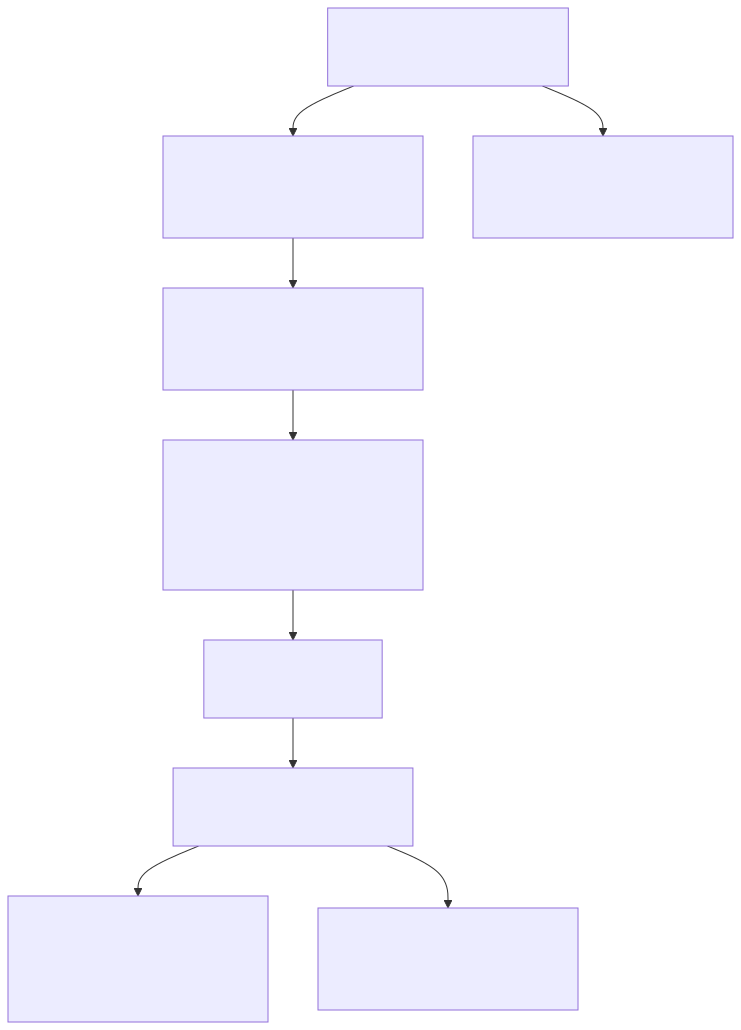
\includegraphics[width=\maxwidth,keepaspectratio,alt={Mermaid Diagram 1}]{0007-economic-reward-system/mermaid_1.png}}
\caption{Mermaid Diagram 1}
\end{figure}

\subsection{5. Data Collection and
Enrichment}\label{data-collection-and-enrichment}

\subsubsection{5.1 Data Sources}\label{data-sources}

Data is gathered from multiple sources to build a comprehensive view of
the network and its participants. The HOPR node API provides a list of
currently visible peers and the network topology, including open payment
channels and their balances. Subgraphs supply information about
registered nodes and their associated Safes. Direct RPC calls are used
to provide specific allocations to targeted accounts (which may increase
a peer's effective stake) and to retrieve those accounts' EOA balances.
Finally, a static list of NFT owners is used to allow reward
distribution to individuals holding a special ``OG NFT''. This
combination of sources ensures that both the live state of the network
and relevant historical or off-chain data are considered in the reward
process.

\subsubsection{5.2 Data Enrichment}\label{data-enrichment}

Once collected, the data is used to enrich each peer object. Registered
node information is used to associate each peer with a Gnosis Safe and
other node metadata. Allocations and EOA balances are incorporated to
adjust the peer's effective stake and balance, reflecting both on-chain
and off-chain holdings. The network topology data is used to determine
the peer's channel balance, which is important for both eligibility and
reward calculation. It is important to note that NFT holder status and
CT node status are not directly added to the peer object during
enrichment. Instead, these are checked during the eligibility filtering
phase.

The following diagram illustrates the data enrichment process:

\begin{figure}
\centering
\pandocbounded{\includegraphics[width=\maxwidth,keepaspectratio,alt={Mermaid Diagram 2}]{0007-economic-reward-system/mermaid_2.png}}
\caption{Mermaid Diagram 2}
\end{figure}

\subsection{6. Peer eligibility
filtering}\label{peer-eligibility-filtering}

The eligibility filtering process is designed to ensure that only peers
who are meaningfully participating in the network and contributing
resources are considered for rewards. The first filter checks that the
peer's safe allowance meets a minimum threshold, ensuring that only
active and funded peers are included. Next, the system excludes any peer
that is also a CT node to prevent self-rewarding. The NFT/stake
requirement is then applied: if a peer is not an NFT holder, they must
meet a higher minimum stake threshold, while NFT holders may be subject
to a lower threshold. Finally, all peers must meet a minimum stake
requirement, regardless of NFT status. Only those who pass all these
checks are considered eligible for rewards.

The following flowchart details the filtering logic:

\begin{figure}
\centering
\pandocbounded{\includegraphics[width=\maxwidth,keepaspectratio,alt={Mermaid Diagram 3}]{0007-economic-reward-system/mermaid_3.png}}
\caption{Mermaid Diagram 3}
\end{figure}

\subsection{7. Economic Model
Application}\label{economic-model-application}

For each eligible peer, the system applies an economic model---such as a
sigmoid or legacy model---to determine the number of messages (reward
units) they should receive over the course of a year. The model takes
into account the peer's individual stake, the total network stake, the
network's capacity, and historical activity metrics such as message
relay counts. The output of this model is the yearly message count for
each peer, which directly determines their share of rewards.

The following diagram shows the economic model application:

\begin{figure}
\centering
\pandocbounded{\includegraphics[width=\maxwidth,keepaspectratio,alt={Mermaid Diagram 4}]{0007-economic-reward-system/mermaid_4.png}}
\caption{Mermaid Diagram 4}
\end{figure}

\subsection{8. Message Timing and Delay
Calculation}\label{message-timing-and-delay-calculation}

The timing between messages sent to each eligible peer is carefully
calculated to ensure a fair and even distribution throughout the year.
The base delay between two messages is computed as the total number of
seconds in a non-leap year divided by the peer's yearly message count.
To allow for efficient batching and aggregation, the system introduces
two session parameters: \codebubble{aggregated\_packets} and
\codebubble{batch\_size}. The actual sleep time between message batches
is the product of the base delay, the number of aggregated packets, and
the batch size. This approach allows the system to send bursts of
messages followed by a pause, balancing throughput and network load. The
values of these parameters can be tuned to optimise performance and
reliability.

The \codebubble{aggregated\_packets} parameter specifies how many
messages are grouped together and sent in a single relay operation,
while \codebubble{batch\_size} determines how many such operations are
performed before the system waits for the next delay interval. The
product of these two parameters gives the total number of messages sent
in each cycle, and the delay is applied after each cycle. This mechanism
provides fine-grained control over the message sending pattern.

\subsection{9. Message Sending
Architecture}\label{message-sending-architecture}

When it is time to send messages, the system first establishes a UDP
session for each eligible peer, selecting a destination CT node at
random (excluding the local node). Each session is managed by a
\codebubble{SessionToSocket} object, which handles both the session
metadata and the underlying UDP socket. The socket is configured with
appropriate buffer sizes and is closed when the session ends to prevent
resource leaks.

Messages themselves are constructed using the \codebubble{MessageFormat}
class, which encodes all necessary metadata---such as sender, relayer,
packet size, and indices---into a raw byte string. The message is padded
to the required packet size and sent through the UDP socket to the
destination node's address and port. The system can optionally wait for
a response to measure round-trip time, which is useful for monitoring
and diagnostics.

The batching of multiple message sendings is handled according to the
session parameters described earlier. Multiple messages can be sent in a
batch, and after each batch, the system waits for the calculated delay
before sending the next batch. This approach ensures that message
delivery is both efficient and aligned with the reward allocation
determined by the economic model.

The following flowchart summarizes the message sending process:

\begin{figure}
\centering
\pandocbounded{\includegraphics[width=\maxwidth,keepaspectratio,alt={Mermaid Diagram 5}]{0007-economic-reward-system/mermaid_5.png}}
\caption{Mermaid Diagram 5}
\end{figure}

\subsection{10. Security and Monitoring}\label{security-and-monitoring}

Security and monitoring are integral to the HOPR CT reward distribution
process. To ensure transparency and facilitate troubleshooting, all
delays and message counts are tracked using Prometheus metrics. This
allows operators and developers to monitor the system's performance in
real time, detect anomalies, and analyse historical trends.

Resource management is also a key concern. The system is designed to
manage sessions and sockets carefully, ensuring that resources are
allocated and released appropriately. Sockets are closed when sessions
end, and sessions are only maintained for as long as they are needed.
This approach helps prevent resource leaks, which could otherwise
degrade system performance or cause failures over time.

Finally, the system enforces strict eligibility checks before sending
messages. Only peers that have open payment channels and valid, active
sessions are eligible to receive messages. This ensures that rewards are
distributed only to those who are actively participating in the network
and have met all necessary criteria, further enhancing the security and
integrity of the reward process.

\subsection{11. Appendix: Data
Structures}\label{appendix-data-structures}

\subsubsection{Registered Node}\label{registered-node}

\begin{longtable}[]{@{}
  >{\raggedright\arraybackslash}p{(\linewidth - 4\tabcolsep) * \real{0.2255}}
  >{\raggedright\arraybackslash}p{(\linewidth - 4\tabcolsep) * \real{0.0784}}
  >{\raggedright\arraybackslash}p{(\linewidth - 4\tabcolsep) * \real{0.6961}}@{}}
\toprule\noalign{}
\begin{minipage}[b]{\linewidth}\raggedright
Variable Name
\end{minipage} & \begin{minipage}[b]{\linewidth}\raggedright
Type
\end{minipage} & \begin{minipage}[b]{\linewidth}\raggedright
Purpose
\end{minipage} \\
\midrule\noalign{}
\endhead
\bottomrule\noalign{}
\endlastfoot
address & str & Node's unique address \\
safe & Safe & Associated Gnosis Safe object \\
\ldots{} & \ldots{} & (Other metadata as provided by subgraph) \\
\end{longtable}

\clearpage

\subsubsection{Safe}\label{safe}

\begin{longtable}[]{@{}
  >{\raggedright\arraybackslash}p{(\linewidth - 4\tabcolsep) * \real{0.2772}}
  >{\raggedright\arraybackslash}p{(\linewidth - 4\tabcolsep) * \real{0.1089}}
  >{\raggedright\arraybackslash}p{(\linewidth - 4\tabcolsep) * \real{0.6139}}@{}}
\toprule\noalign{}
\begin{minipage}[b]{\linewidth}\raggedright
Variable Name
\end{minipage} & \begin{minipage}[b]{\linewidth}\raggedright
Type
\end{minipage} & \begin{minipage}[b]{\linewidth}\raggedright
Purpose
\end{minipage} \\
\midrule\noalign{}
\endhead
\bottomrule\noalign{}
\endlastfoot
address & str & Safe contract address \\
balance & Balance & Total balance held in the safe \\
allowance & Balance & Allowance available for node operations \\
additional\_balance & Balance & Extra balance from allocations/EOA \\
owners & list & List of owner addresses \\
\ldots{} & \ldots{} & (Other metadata as provided by subgraph) \\
\end{longtable}

\subsubsection{Allocation}\label{allocation}

\begin{longtable}[]{@{}
  >{\raggedright\arraybackslash}p{(\linewidth - 4\tabcolsep) * \real{0.2673}}
  >{\raggedright\arraybackslash}p{(\linewidth - 4\tabcolsep) * \real{0.1188}}
  >{\raggedright\arraybackslash}p{(\linewidth - 4\tabcolsep) * \real{0.6139}}@{}}
\toprule\noalign{}
\begin{minipage}[b]{\linewidth}\raggedright
Variable Name
\end{minipage} & \begin{minipage}[b]{\linewidth}\raggedright
Type
\end{minipage} & \begin{minipage}[b]{\linewidth}\raggedright
Purpose
\end{minipage} \\
\midrule\noalign{}
\endhead
\bottomrule\noalign{}
\endlastfoot
address & str & Allocation contract address \\
unclaimed\_amount & Balance & Amount not yet claimed \\
linked\_safes & set & Safes associated with this allocation \\
num\_linked\_safes & int & Number of safes linked \\
\end{longtable}

\subsubsection{EOA Balance}\label{eoa-balance}

\begin{longtable}[]{@{}
  >{\raggedright\arraybackslash}p{(\linewidth - 4\tabcolsep) * \real{0.3039}}
  >{\raggedright\arraybackslash}p{(\linewidth - 4\tabcolsep) * \real{0.1373}}
  >{\raggedright\arraybackslash}p{(\linewidth - 4\tabcolsep) * \real{0.5588}}@{}}
\toprule\noalign{}
\begin{minipage}[b]{\linewidth}\raggedright
Variable Name
\end{minipage} & \begin{minipage}[b]{\linewidth}\raggedright
Type
\end{minipage} & \begin{minipage}[b]{\linewidth}\raggedright
Purpose
\end{minipage} \\
\midrule\noalign{}
\endhead
\bottomrule\noalign{}
\endlastfoot
address & str & EOA address \\
balance & Balance & Balance held by the EOA \\
linked\_safes & set & Safes associated with this EOA \\
num\_linked\_safes & int & Number of safes linked \\
\end{longtable}

\clearpage

\subsubsection{Topology Entry}\label{topology-entry}

\begin{longtable}[]{@{}
  >{\raggedright\arraybackslash}p{(\linewidth - 4\tabcolsep) * \real{0.2843}}
  >{\raggedright\arraybackslash}p{(\linewidth - 4\tabcolsep) * \real{0.1275}}
  >{\raggedright\arraybackslash}p{(\linewidth - 4\tabcolsep) * \real{0.5882}}@{}}
\toprule\noalign{}
\begin{minipage}[b]{\linewidth}\raggedright
Variable Name
\end{minipage} & \begin{minipage}[b]{\linewidth}\raggedright
Type
\end{minipage} & \begin{minipage}[b]{\linewidth}\raggedright
Purpose
\end{minipage} \\
\midrule\noalign{}
\endhead
\bottomrule\noalign{}
\endlastfoot
address & str & Peer address \\
channels\_balance & Balance & Total balance in outgoing channels \\
\end{longtable}

\subsubsection{Peer (Enriched)}\label{peer-enriched}

\begin{longtable}[]{@{}
  >{\raggedright\arraybackslash}p{(\linewidth - 4\tabcolsep) * \real{0.3431}}
  >{\raggedright\arraybackslash}p{(\linewidth - 4\tabcolsep) * \real{0.1765}}
  >{\raggedright\arraybackslash}p{(\linewidth - 4\tabcolsep) * \real{0.4804}}@{}}
\toprule\noalign{}
\begin{minipage}[b]{\linewidth}\raggedright
Variable Name
\end{minipage} & \begin{minipage}[b]{\linewidth}\raggedright
Type
\end{minipage} & \begin{minipage}[b]{\linewidth}\raggedright
Purpose
\end{minipage} \\
\midrule\noalign{}
\endhead
\bottomrule\noalign{}
\endlastfoot
address & Address & Peer's unique address \\
version & Version & Peer's software version \\
safe & Safe & Associated safe object \\
channel\_balance & Balance & Balance in outgoing channels \\
yearly\_message\_count & int/None & Calculated reward allocation \\
params & Parameters & Application parameters \\
running & bool & Is the peer currently active \\
\ldots{} & \ldots{} & (Other runtime attributes) \\
\end{longtable}

\subsection{12. References}\label{references}

{[}01{]} Bradner, S. (1997).
\href{https://datatracker.ietf.org/doc/html/rfc2119}{Key words for use
in RFCs to Indicate Requirement Levels}. \emph{IETF RFC 2119}.

\subsection{13. Changelog}\label{changelog}

\begin{itemize}
\tightlist
\item
  2025-06-26: Initial draft.
\end{itemize}
